\documentclass[a4paper,11pt, draft]{article}

\usepackage[finnish]{babel}
\usepackage[utf8]{inputenc}
\usepackage[margin=2cm]{geometry}
\usepackage{amsfonts,amsmath,amssymb,amsthm,enumitem}
\usepackage{microtype}
\usepackage{array}
\usepackage{booktabs}
\usepackage{pgf}
\usepackage{tikz}
\usepackage{tikz-qtree}
\usetikzlibrary{arrows,automata}

\setenumerate{listparindent=\parindent}

\newtheorem*{claim}{Väite}

\newcommand{\set}[1]{{\left\{ #1 \right\}}}
\newcommand{\ceil}[1]{{\left\lceil#1\right\rceil}}
\newcommand{\Nat}{\mathbb{N}}
\newcommand{\ve}{\varepsilon}

\newenvironment{automata}[1][2.8]%
{\begin{tikzpicture}[->,>=stealth',shorten >=1pt,auto,node distance=#1cm,semithick]}%
{\end{tikzpicture}}

\newenvironment{centerautomata}[1][2.8]%
{\begin{center}\begin{automata}[#1]}%
{\end{automata} \end{center}}

\newcolumntype{W}{>{\centering\arraybackslash}m{5cm} }
\newcolumntype{V}{>{\centering\arraybackslash}m{2cm} }

\begin{document}

\subsection*{582206 Laskennan mallit, syksy 2012 \\
  \textmd{7. harjoitusten malliratkaisut \\
    Juhana Laurinharju ja Jani Rahkola}}

\begin{enumerate}
  \item
    Esitä pinoautomaatti seuraaville kielille.
    \begin{enumerate}
      \item
        Kaikki palindromit aakkostosta $\Sigma = \set{a, b, c}$.

        \begin{centerautomata}
            \node[initial, state] (q0) {$q_0$};
            \node[state] (q1) [right of=q0] {$q_1$};
            \node[state] (q2) [right of=q1] {$q_2$};
            \node[state, accepting] (q3) [right of=q2] {$q_3$};

            \path
            (q0) edge node {$\ve, \ve \to \$ $} (q1)
            (q1) edge [loop below] node {$\begin{aligned}
                              a, \ve \to a \\
                              b, \ve \to b \\
                              c, \ve \to c
                            \end{aligned}$} (q0)
            (q1) edge node {$\begin{aligned}
                                \ve, \ve \to \ve\\
                                a, \ve \to \ve \\
                                b, \ve \to \ve \\
                                c, \ve \to \ve
                            \end{aligned}$} (q2)
            (q2) edge [loop below] node {$\begin{aligned}
                                a, a \to \ve \\
                                b, b \to \ve \\
                                c, c \to \ve
                            \end{aligned}$} (q2)
            (q2) edge node {$\ve, \$ \to \ve$} (q3);

        \end{centerautomata}

      \item
        $\set{a^ib^j \mid 0 \le i \le j}$ missä $\Sigma = \set{a, b, c}$

        \begin{centerautomata}
            \node[initial, state] (q0) {$q_0$};
            \node[state] (q1) [right of=q0] {$q_1$};
            \node[state] (q2) [right of=q1] {$q_2$};
            \node[state] (q3) [right of=q2] {$q_3$};

            \path
            (q0) edge node {$\ve, \ve \to \$ $} (q1)
            (q1) edge [loop below] node {$a, \ve \to 1$} (q1)
            (q1) edge node {$\ve, \ve \to \ve$} (q2)
            (q2) edge [loop below] node {$b, 1 \to \ve$} (q2)
            (q2) edge node {$\ve, \$ \to \ve$} (q3)
            (q3) edge [loop below] node {$b, \ve \to \ve$} (q3);
        \end{centerautomata}

      \item
        $\set{a^ib^jc^k \mid j = i + k}$ missä $\Sigma = \set{a, b, c}$

        \begin{centerautomata}
            \node[initial, state] (q0) {$q_0$};
            \node[state] (q1) [above of=q0] {$q_1$};
            \node[state] (q2) [right of=q1] {$q_2$};
            \node[state] (q3) [right of=q2] {$q_3$};
            \node[state] (q4) [right of=q3] {$q_4$};
            \node[state, accepting] (q5) [below of=q4] {$q_5$};

            \path
            (q0) edge node {$\ve, \ve \to \$ $} (q1)
            (q1) edge [loop above] node {$a, \ve \to 1$} (q1)
            (q1) edge node {$\ve, \ve \to \ve$} (q2)
            (q2) edge [loop above] node {$b, 1 \to \ve$} (q2)
            (q2) edge node {$\ve, \$ \to \$ $} (q3)
            (q3) edge [loop above] node {$b, \ve \to 1$} (q3)
            (q3) edge node {$\ve, \ve \to \ve$} (q4)
            (q4) edge [loop above] node {$c, 1 \to \ve$} (q4)
            (q4) edge node {$\ve, \$ \to \ve$} (q5) ;
        \end{centerautomata}

      \item
        Kaikki aakkoston $\Sigma = \set{0, 1}$ merkkijonot joissa nollia on
        kaksi kertaa niin paljon kuin ykkösiä.

        \begin{centerautomata}[3]
          \node[state] (q1) {$q_1$};
          \node[state] (q2) [below of=q1] {$q_2$};
          \node[state] (q3) [above of=q1] {$q_3$};
          \node[initial,state] [left of=q3] (q0) {$q_0$};
          \node[state] (q5) [right of=q3] {$q_5$};
          \node[state] (q4) [right of=q5] {$q_4$};
          \node[state, accepting] (q6) [left of=q2] {$q_6$};

          \path
          (q0) edge [bend right=40] node [swap] {$\ve, \ve \to \$$} (q1)
          (q1) edge [bend right=40] node [swap] {$\ve, \$ \to \ve$} (q6)
          (q1) edge [out=350, in=320, looseness=10] node {$0, A \to \ve$} (q1)
          (q1) edge [bend left=15] node {$1, Y \to \ve$} (q3)
          (q3) edge [bend left=15] node {$\ve, Y \to \ve$} (q1)
          (q1) edge [bend right,looseness=1.3] node [swap] {$\begin{aligned}
                             1&, \$ \to \$ \\
                             1&, A \to A
                           \end{aligned}$} (q4)
          (q3) edge node {$\ve, \$ \to \$$} (q5)
          (q4) edge node [swap] {$\ve, \ve \to A$} (q5)
          (q5) edge [bend left,looseness=1.2] node {$\ve, \ve \to A$} (q1)
          (q1) edge [bend right=15] node [swap] {$\begin{aligned}
                                         0&, \$ \to \$ \\
                                         0&, Y \to Y
                                       \end{aligned}$} (q2)
          (q2) edge [bend right=15] node [swap] {$\ve, \ve \to Y$} (q1);
        \end{centerautomata}

        Automaatin ideana on pitää pinossa kirjaa siitä kuinka paljon
        nolla-merkkien määrässä on yli- tai alijäämää. Pinoon laitetaan $A$
        jos siirtymä kerryttää alijäämää ja $Y$ jos se kerryttää ylijäämää.
        Vastaavasti pinosta poistetaan merkkejä aina tilaisuuden tullen, kun
        syötemerkin lukeminen tasoittaa nollien ja ykkösten suhdetta.
    \end{enumerate}

  \item
    Tarkastellaan kielioppia
%
    \begin{align*}
      S & \to S+T \mid T \\
      T & \to T*F \mid F \\
      F & \to (S) \mid a
    \end{align*}
%
    Muodosta merkkijonon $s=( a+ a)* a$ jäsennyspuu tämän kieliopin
    mukaisesti.

    Etsi jäsennyspuusta jokin juuresta lehteen johtava polku, jolla sama
    muuttuja esiintyy kahdessa solmussa. Muodosta tämän perusteella
    toistuvuusominaisuuden todistuksen ideaa mukaillen jokin merkkijonon $s$
    jako osiin $s=uvxyz$, joilla merkkijono $uv^ixy^iz$ kuuluu tarkasteltavaan
    kieleen kaikilla $i\in N$.

    \begin{center}
      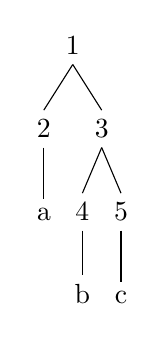
\begin{tikzpicture}
        {\Tree [.1 [.2 a ] [.3 [.4 b ] [.5 c ] ] ]}
      \end{tikzpicture}
    \end{center}

  \item
    Olkoon $A$ aakkoston $\set{0,1}$ kieli, joka koostuu niistä
    merkkijonoista, joissa on sama määrä nollia ja ykkösiä. Tällä kielellä on
    kontekstiton kielioppi
%
    \begin{equation*}
      S \to SS \mid 0S1 \mid 1S0 \mid \ve
    \end{equation*}
%
    \begin{enumerate}
    \item
      Kielen $A$ eräs toistuvuuspituus on 4. Esitä kieleen $A$ kuuluvalle
      merkkijonolle $s=001101$ kaikki eri tavat jakaa se osiin $s=uvxyz$
      toistuvuusominaisuuden ehdot toteuttavalla tavalla (lause 2.30; Sipser
      Theorem 2.34; tässä siis $p=4$).

      \begin{center}
        \begin{tabular}{ccccc}
          \toprule
          $u$         & $v$  & $x$ & $y$  & $z$ \tabularnewline
          \midrule
          &      &     & 0011 & 01\tabularnewline
          &      & 0   & 01   & 101\tabularnewline
          & 0    &     & 011  & 01\tabularnewline
          & 0    & 0   & 1    & 101\tabularnewline
          & 0    & 01  & 1    & 01\tabularnewline
          & 00   &     & 11   & 01\tabularnewline
          & 001  &     & 1    & 01\tabularnewline
          & 0011 &     &      & 01\tabularnewline
          0           &      &     & 01   & 101\tabularnewline
          0           &      &     & 0110 & 1\tabularnewline
          0           &      & 01  & 10   & 1\tabularnewline
          0           & 0    &     & 1    & 101\tabularnewline
          0           & 0    &     & 110  & 1\tabularnewline
          0           & 0    & 1   & 1    & 01\tabularnewline
          0           & 01   &     &      & 101\tabularnewline
          0           & 01   &     & 10   & 1\tabularnewline
          0           & 01   & 1   &      & 01\tabularnewline
          0           & 01   & 10  &      & 1\tabularnewline
          0           & 011  &     & 0    & 1\tabularnewline
          0           & 0110 &     &      & 1\tabularnewline
          00          &      & 1   & 10   & 1\tabularnewline
          00          &      & 11  & 01   & \tabularnewline
          00          & 1    & 1   & 0    & 1\tabularnewline
          001         &      &     & 10   & 1\tabularnewline
          001         &      & 1   & 01   & \tabularnewline
          001         & 1    &     & 0    & 1\tabularnewline
          001         & 10   &     &      & 1\tabularnewline
          001         & 10   & 1   &      & \tabularnewline
          0011        &      &     & 01   & \tabularnewline
          0011        & 0    &     & 1    & \tabularnewline
          0011        & 01   &     &      & \tabularnewline
          \bottomrule
        \end{tabular}
      \end{center}

      Yhteensä 31 ehdot täyttävää jakoa.

    \item
      Onko kielellä $A$ pienempiä toistuvuuspituuksia kuin 4? Perustele.
    \end{enumerate}

  \item
    \begin{enumerate}
      \item
        Koostukoon aakkoston $\set{a,b,c}$ kieli $A$ merkkijonoista, joissa on
        yhtä monta $a$-, $b$- ja $c$-merkkiä.
        \begin{claim}
          Kieli $A$ ei ole yhteydetön.
        \end{claim}
        \begin{proof}
          Oletetaan vastoin väitettä, että kieli $A$ on yhteydetön. Nyt
          tehtävässä 7 todistetun nojalla leikkaus $A \cap L(a^*b^*c^*) =
          \set{a^nb^nc^n \mid n \in \Nat}$ on yhteydetön. Tämä on kuitenkin
          tunnetusti ristiriita. Siis kieli $A$ ei ole yhteydetön.
        \end{proof}

      \item
        Osoita, että kieli $\set{0^n1^n0^n1^n \mid n \in \Nat}$ ei ole
        yhteydetön.
        \begin{claim}
          Kieli $A = \set{0^n1^n0^n1^n \mid n \in \Nat}$ ei ole yhteydetön.
        \end{claim}
        \begin{proof}
          Oletetaan vastoin väitettä, että kieli $A$ on yhteydetön. Nyt
          pumppauslemman nojalla sillä on pumppauspituus $p$. Valitaan
          merkkijono $s = 0^p1^p0^p1^p$. Nyt merkkijonon jakojen $s = uvxyz$
          tulisi täyttää pumppauslemman ehdot.

          Merkkijonon $s$ pituus on $4p$ ja koska osaan $vxy$ ei saa tulla yli
          $p$:tä merkkiä, täytyy osiin $u$ ja $z$ jäädä yhteensä vähintään
          $3p$ merkkiä. Nyt siis joko osaan $u$ jäävät ainakin kaikki
          merkkijonon $p$ esimmäistä nollaa, tai osaan $z$ jäävät ainakin
          kaikki merkkijonon $p$ viimeistä ykköstä.

          Jos kieleen $A$ kuuluvassa merkkijonossa on $p$ kappaletta
          peräkkäisiä nollia tai $p$ kappaletta peräkkäisiä ykkösiä, täytyy
          merkkijonon pituuden olla $4p$. Pumppauslemman mukaan merkkijonon
          $uv^0xy^0z = uxz$ tulisi kuulua kieleen $A$. Koska osat $u$ ja $z$
          pitävät sisällään joko $p$ nollaa tai $p$ ykköstä, tulisi
          merkkijonon $uxz$ pituuden olla edelleen $4p$ jotta se voisi kuulua
          kieleen $A$. Koska puuttuvat osat $v$ ja $y$ eivät kuitenkaan
          saaneet molemmat olla tyhjiä, täytyy merkkijonon $uxz$ pituuden olla
          aidosti vähemmän kuin $4p$. Siis $uxz$ ei kuulu kieleen $A$, mikä on
          ristiriita. Täten kieli $A$ ei ole yhdeydetön.
        \end{proof}
    \end{enumerate}

  \item
    Anna yhteydetön kielioppi, joka tuottaa kielen $\set{a^ib^jc^k \mid i = 2j
      \text{ tai } j = 2k}$. Muodosta a\-pu\-lau\-seen 2.21 mukaisesti
    kieliopistasi pinoautomaatti, joka tunnistaa saman kielen.

    \begin{align*}
      S & \to T_{aab}T_c \mid T_a T_{bbc} \\
      T_{aab} & \to aaT_{aab}b \mid \ve \\
      T_c & \to cT_c \mid \ve \\
      T_a & \to aT_a \mid \ve \\
      T_{bbc} & \to bbT_{bbc}c \mid \ve
    \end{align*}

  \item
    Tee alla olevasta pinoautomaatista Apulauseen 2.27 mukaisesti kielioppi.

    \begin{centerautomata}
      \node[initial,state,accepting]   (q0)                     {$q_0$};
      \node[state]           (q1) [above right of=q0] {$q_1$};
      \node[state,accepting] (q3) [below right of=q0] {$q_3$};
      \node[state]           (q2) [above right of=q3] {$q_2$};

      \path (q0) edge              node {$\ve, \ve \to \$ $} (q1)
            (q1) edge [loop above] node {$\begin{aligned}
                                           0, & \ve \to  0 \\
                                           1, & \ve \to  1
                                         \end{aligned}$} ()
                 edge              node {$\ve,\ve\to\ve$} (q2)
            (q2) edge [loop right] node {$\begin{aligned}
                                          0, & 0 \to \ve \\
                                          1, & 1 \to \ve
                                          \end{aligned}$} ()
                 edge              node {$\ve,\$ \to \ve$} (q3);
    \end{centerautomata}

  \item
    \begin{enumerate}
    \item
      Osoita, että jos $A$ on yhteydetön ja $B$ säännöllinen kieli, niin
      $A\cap B$ on yhteydetön.

      \emph{Vihje:} muodosta pinoautomaatin ja äärellisen automaatin
      leikkausautomaatti samaan tapaan kuin Jyrkin luentojen lauseessa 1.1
      (luentomateriaalin sivut 48--50).

      Olkoon $A$ yhteydetön kieli ja $M_A = (Q_A, \Sigma, \Gamma, \delta_A,
      q_{A0}, F_A)$ automaatti joka tunnistaa kielen $A$. Olkoon $B$
      säännöllinen kieli ja $M_B = (Q_B, \Sigma, \delta_B, q_{B0}, F_B)$
      deterministinen automaatti joka tunnistaa kielen $B$.
      \begin{claim}
         Kieli $A \cap B$ on säännöllinen.
      \end{claim}
      \begin{proof}
        Leikkauksen tunnistava automaatti luodaan samankaltaisella
        menetelmällä kuin säännöllisten kielten tapauksessa. Ero säännöllisten
        kielten tapaukseen on siirtymäfunktion $\delta_{A \cap B}$
        määrrittelyssä.

        Muodostetaan siis automaatti
        \begin{equation*}
          M_{A \cap B} = (Q_A \times Q_B \text{, } \Sigma \text{, } \Gamma
          \text{, } \delta_{A \cap B} \text{, } (q_{A0}, q_{B0}) \text{, } F_A
          \times F_B)
        \end{equation*}
        missä siirtymäfunktio $\delta_{A \cap B}$ on määritelty seuraavasti.
%
        \begin{equation*}
          \delta_{A \cap B}((q_i, p_i), a, t) = 
          \begin{cases}
            \{((q_j, p_i),s) \mid \delta_A(q_i, \ve, t) = (q_j, s)\} & \text{
              kun } a = \ve \\

            \{((q_j, p_j),s) \mid \delta_B(q_i, a) = q_j \text{ ja }
            \delta_A(p_i, a, t) = (p_j, s)\} & \text{ muulloin}
          \end{cases}
        \end{equation*}
%
        Kaikki uuden automaatin tilat ovat siis muotoa $(q, p)$ missä $q \in
        Q_A$ ja $p \in Q_B$. Siirtymät noudattavat parin ensimmäisen alkion
        kohdalla automaatin $M_A$ siirtymäfunktiota ja toisen alkion kohdalla
        automaatin $M_B$ siirtymäfunktiota. Pinon käsittely noudattaa aina
        automaatin $M_A$ siirtymäfunktiota, sillä automaatissa $M_B$ ei ole
        pinoa.
%
        \begin{center}
        \begin{tabular}{W V W}
        \begin{automata}
          \node[state] (qi)               {$q_i$};
          \node[state] (qj) [right of=qi] {$q_j$};

          \path (qi) edge node {$a, t \to s$} (qj);
        \end{automata} & & \tabularnewline
        &
        \scalebox{2}{$\to$}
        &
        \begin{automata}[3.5]
          \tikzstyle{every state}=[shape=rectangle, rounded corners];
          \node[state] (i) {$(q_i, p_i)$};
          \node[state] (j) [right of=i] {$(q_j, p_j)$};

          \path (i) edge node {$a, t \to s$} (j);
        \end{automata} \tabularnewline
        \begin{automata}
          \node[state] (pi)               {$p_i$};
          \node[state] (pj) [right of=pi] {$p_j$};

          \path (pi) edge node {$a$} (pj);
        \end{automata} & &
        \end{tabular}
        \end{center}
%
        Pinoautomaatti $M_A$ on e\-pä\-de\-ter\-mi\-nis\-ti\-nen, mutta $M_B$
        ei. Pinoautomaatin e\-pä\-de\-ter\-mi\-nis\-tis\-ten siirtymien
        kohdalla uudessa automaatissa tilaparin jälkimmäinen alkio ei muutu.
        Ensimmäinen alkio noudattaa pinoautomaatin $M_A$ siirtymäfunktiota.
%
        \begin{center}
        \begin{tabular}{W V W}
        \begin{automata}
          \node[state] (qi)               {$q_i$};
          \node[state] (qj) [right of=qi] {$q_j$};
 
          \path (qi) edge node {$\ve, t \to s$} (qj);
         \end{automata}
        &
        \scalebox{2}{$\to$}
        &
        \begin{automata}[3.5]
          \tikzstyle{every state}=[shape=rectangle, rounded corners];
          \node[state] (i) {$(q_i, p_i)$};
          \node[state] (j) [right of=i] {$(q_j, p_i)$};

          \path (i) edge node {$\ve, t \to s$} (j);
        \end{automata}
        \end{tabular}
        \end{center}
%
        Luotu automaatti $M_{A \cap B}$ hyväksyy merkkijonon $w$ jos ja vain
        jos $M_A$ ja $M_B$ hyväksyvät merkkijonon $w$. Siis $M_{A \cap B}$
        tunnistaa kielen $A \cap B$.
      \end{proof}

    \item
      Tiedetään, että kieli $L$ on yhteydetön ja $R$ säännöllinen. Voidaanko
      tästä päätellä, että $L-R$ on yhteydetön? Entä $R-L$? Perustele.

      \begin{claim}
        Olkoon $L$ yhteydetön ja $R$ säännöllinen kieli. Nyt $L - R$ on
        yhteydetön.
      \end{claim}
      \begin{proof}
        Joukko-opista tiedämme, että $L - R = L \cap \overline{R}$. Lisäksi
        tiedämme, että säännölliset kielet ovat suljettuja komplementin
        suhteen. Nyt siis edellisen kohdan nojalla $L \cap \overline{R}$ on
        yhteydetön, ja siten myös $L - R$ on yhteydetön.
      \end{proof}

      Toinen suunta ei päde yleisesti. Koska yhteydettömät kielet eivät ole
      suljettuja komplementin suhteen, on olemassa yhteydetön kieli jonka
      komplementti ei ole yhteydetön. Olkoon $L$ jokin tällainen kieli. Olkoon
      nyt $R = \Sigma^*$ joka tunnetusti säännöllinen. Nyt siis $L$ on
      yhteydetön ja $R$ säännöllinen, mutta $R - L = \Sigma^* - L =
      \overline{L}$ joka oletuksen mukaan ei ole yhteydetön.
    \end{enumerate}
\end{enumerate}

\end{document}
